
\chapter{Background and Observation Errors} % Main chapter title

\label{chap:bandoerrs} % For referencing the chapter elsewhere, use \ref{Chapter1} 

This chapter contains a discussion of the background and observation errors in our DA system. Though the background errors are determined directly from the ensemble when using the ETKF method, understanding the form they take is crucial to understanding how the DA system works. This is because, according to equation \ref{eqn:analysisupdate}, the DA increments always lie in the column space of the background error covariance matrix. This means that the background errors determine how information from the observations can be propagated around the domain by DA.

The observation errors are also important to understanding a DA system since the balance between observation and background errors determines how much weight is given to the observations by the DA. The observation errors must be estimated manually, and a description of the methods used to do this are included here.

%----------------------------------------------------------------------------------------
%	SECTION 1
%----------------------------------------------------------------------------------------

\section{Background Errors}
\label{sec:bgerrors}

In our case the background error covariance matrix is approximated by the forecast error covariance matrix $\mat{P}^f$, defined in equation \ref{eqn:ferrorcov}. The elements of $\mat{P}^f$ are the ensemble covariances at each pair of gridpoints and timesteps,

\begin{equation}
\mat{P}^f_{ij} = \text{cov}\left( \x^f_i, \x^f_j \right),
\end{equation}

where $\x^f_i$ refers here to the ensemble values in component $i$ of the state vector. The diagonal elements are then the ensemble variance at each gridpoint and timestep:

\begin{equation}
\mat{P}^f_{ii} = \text{var}\left( \x^f_i \right).
\end{equation}

Figure \ref{fig:hsensseries} shows a timeseries of $H_s$ ensemble mean and variance at the buoy location from the forecast starting 12Z 10/03/2022. A peak on the 12th is apparent as in figure \ref{fig:wavesandchart}. Figure \ref{fig:hsensseries} also shows that the variance is a strong function of the mean. The variance in $H_s$ peaks just before the peak in the mean and drops back to a lower value as the mean reaches its peak. This means that the background error in $H_s$ is highest just before the peak in $H_s$.

Figure \ref{fig:t01ensseries} shows the same as  \ref{fig:hsensseries} but for $T_{m01}$. Again it shows a peak in the variance just before the peak in the mean. In this case the peak in $T_{m01}$ is preceded by a dip, and this dip is also associated with a peak in the ensemble variance. This means that the background error variance in $T_{m01}$ is high for a period of $\sim 24$ hours, as opposed to $\sim 12$ hours for $H_s$.

\begin{figure}[h]
	\centering
	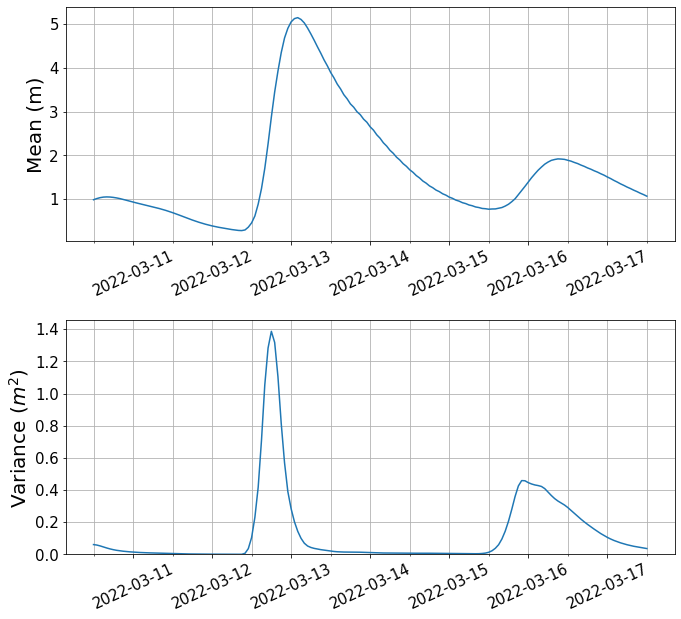
\includegraphics[width = .8\textwidth]{Figures/buoyhsvar}
	\caption{Timeseries of forecast significant wave height ensemble mean (top) and variance (bottom) at the buoy location from the model run starting on the 10/03/2022.}
	\label{fig:hsensseries}
\end{figure}

\begin{figure}[h]
	\centering
	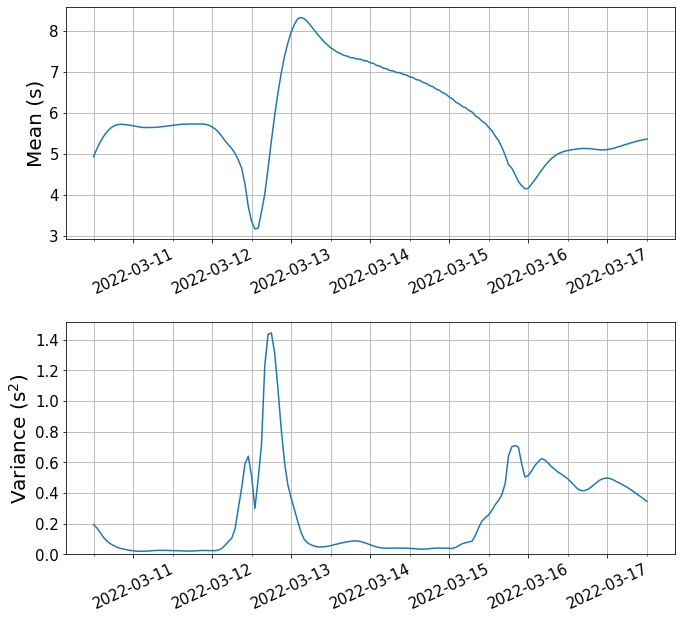
\includegraphics[width = .8\textwidth]{Figures/buoyt01var}
	\caption{Timeseries of forecast $T_{m01}$ ensemble mean (top) and variance (bottom) at the buoy location from the model run starting on the 10/03/2022.}
	\label{fig:t01ensseries}
\end{figure}

We now present maps of the ensemble covariances in order to illustrate the forms these covariances can take and gain insight into the workings of our DA system. Covariances in space will be considered, as well as cross-covariances between different variables and lagged in time. Arrows showing wind/wave direction will be used to explain the form the covariances take.

Figure \ref{fig:covhshs12-0} shows the spatial covariance of $H_s$ at 12Z 12/03/2022. The colours on the map show the covariance between $H_s$ at each point in the domain and $H_s$ at the buoy (marked with a cross). The arrows show the direction and magnitude of the wind, averaged over the preceding 24 hours. The strongest covariances are confined to the western GoM and do not extend very far from the buoy. From the wind arrows, the wind in the region of strong covariance is very low, similar to the wind at the buoy, and that the wind in regions of weak covariance is high.

\begin{figure}
\centering

\includegraphics[width = .5\textwidth]{figures/covhshs12-0}
\caption{Colours showing spatial covariance of significant wave height at the buoy with significant wave height in the field at 12Z 12/03/2022. Arrows showing wind averaged over prior 24 hours.}
\label{fig:covhshs12-0}
\end{figure}

This suggests that the wind forcing plays a role in determining the nature of the ensemble covariances. This is unsurprising since according to \citet{Lefevre2012}, ocean wave prediction is primarily a forcing problem, and so we expect the nature of the forcing to play a major role in determining the properties of the waves. This is the motivation for averaging the wind values over the preceding 24 hour window, since the wind forcing takes time to have an impact on the waves.

The wind forcing can also induce covariances at longer distances. Figure \ref{fig:covhshs11-0} shows the same as \ref{fig:covhshs12-0} but at 12Z 11/03/2022. The difference in magnitude of the covariance from figure \ref{fig:covhshs11-0} is notable. This could be explained by the fact that the variance in $H_s$ at 12Z 11/03/2022 is much smaller than the variance at 12Z 12/03/2022, as seen in figure \ref{fig:hsensseries}. In figure \ref{fig:covhshs11-0}, nonzero covariances are visible far from the buoy in the Northern GoM. These covariances could also be present in figure \ref{fig:covhshs12-0}, but washed out due to the larger overall magnitude of covariance in that figure. The pattern of winds gives a plausible explanation for these long-ditance covariances: the region of positive covariance in the Northeast has weak winds, similar to the vicinity of the buoy, and the region of negative covariance in the Northwest has strong winds.

It is also possible that these long distance covariances are physcially unrealistic. As discussed in section \ref{sec:DApractice}, an inherent limitation in estimating the background error from the ensemble is that a finite ensemble size leads to sampling error in $\mat{P}^f$. This can cause spurious covariances to arise at long distances \citep{Hunt2007}, which can be fixed with localisation. This possibilty is not explored in this study, partly due to the fact that plausible physical explanations exist for the long-distance covariances, but this is something that should be included in future work on the topic.

\begin{figure}[h]
	\centering
	
\includegraphics[width = .5\textwidth]{figures/covhshs11-0}
	\caption{Colours showing spatial covariance of significant wave height at the buoy and significant wave height in the field at 12Z 11/03/2022. Arrows showing wind averaged over prior 24 hours.}
	\label{fig:covhshs11-0}
\end{figure}

Another thing that can cause long-distance covariances is travelling swell waves. Figure \ref{fig:covhshs13-1} shows the $H_s$ covariance at 18Z 13/03/2022 with a one day lag. In other words, expressing $H_s$ as a function of space and time $H_s = H_s(x,y,t)$ we plot

\[
\text{cov}\left( H_s(x_0,y_0,t_0), H_s(x,y,t_0 - 1 \, \text{day}) \right)
\]

for each $x$ and $y$. Here $(x_0,y_0)$ is the position of the buoy, and $t_0$ is 18Z 13/03/2022. This means the $H_s$ ensemble at the buoy is sampled at 18Z 13/03/2022 and the $H_s$ ensemble elsewhere in the domain is sampled at 18Z 12/03/2022, to show the correlation with earlier sea states.  There is a large region of positive covariance spanning the Western GoM and much of the Northern part also. The arrows mark the wave direction at 18Z 13/03/2022, and this shows that waves from the Northwestern GoM travel West and South towards the buoy. This means they are able to influence the sea state at the buoy, which explains the positive covariance.

Another notable aspect of figure \ref{fig:covhshs13-1} is the general magnitude of covariance seen. The maximum covariance seen in figure \ref{fig:covhshs13-1} is 0.03, compared to 0.20 in figure \ref{fig:covhshs12-0}. This is explained by the one day lag used to generate figure \ref{fig:covhshs13-1}. We expect the covariances between two points to decrease the further apart those two points are in time, and this is what we see. This means that we expect the observations assimilated to have more of an impact on the state at times near the observation time.

\begin{figure}[h]
\centering

\includegraphics[width = .5\textwidth]{figures/covhshs13-1}
\caption{Colours showing covariance of significant wave height at the buoy at 18Z 13/03/2022 with significant wave height in the field at 18Z 12/03/2022. Arrows showing wave direction at 18Z 12/03/2022}
\label{fig:covhshs13-1}
\end{figure}

So far we have only examined the covariance of $H_s$ with itself. There are also covariances present between the different variables assimilated in this study, and this is important for the DA. These cross-covariances allow assimilation of one variable to affect other variables than the one assimilated. This will allow the assimilation of $H_s$ alone to impact $T_{m01}$ and $T_{m02}$, and allow the assimilation of all three variables to produce different forecasts of $H_s$ than would be obtained by assimilating $H_s$ alone. It is hoped that these cross-covariances will improve DA performance by allowing each observation assimilated to provide more information than it would in their absence.

\begin{figure}[h]
\centering
\begin{subfigure}{0.49\textwidth}
\centering

\includegraphics[width = \textwidth]{figures/covhst0112-0wav}
\end{subfigure}
\begin{subfigure}{0.49\textwidth}
\centering

\includegraphics[width = \textwidth]{figures/covhst0112-0wnd}
\end{subfigure}
\caption{Cross-covariance between significant wave height at the buoy and $T_{m01}$ in the field at 12Z 12/03/2022. Arrows show wave direction (left) and wind (right).}
\label{fig:covhst0112-0}
\end{figure}

Figure \ref{fig:covhst0112-0} shows the cross-covariance between $H_s$ at the buoy and $T_{m01}$ elsewhere at 12Z 12/03/2022. There is a large area of positive covariance to the Northwest of the buoy, with the wave direction (left plot) pointing mostly towards the buoy in this region. This suggests that the positive covariance may be related to travelling swell waves, since large swell waves with long period in the region Northwest of the buoy could travel towards the buoy and lead to higher waves there. However more investigation is required to determine if this is actually the case.

There are also small patches of strong negative covariance, directly East of the buoy and also South in the 
Pacific ocean. Since there is no obvious difference in the winds in each region to explain this, these negative covariances could be spurious. This is especially true of the negative covariance seen in the Pacific, since there is no way for the waves here to interact directly with the waves at the buoy.

In this section, we have presented maps showing the forms that the forecast error covariances can take, and attempted to explain them by referring to physical explanations from winds and wave directions, and also to sampling error. However, the physical explanations discussed here are quite simple and surface-level, and more investigation would be useful to explain the form of the covariance. Since understanding the physical mechanisms behind the covariances is not completely central to this section's goal of explaining DA performance, it is not explored further here, but it would be a good avenue for future work.

\section{Diagnosis of Observation Errors}
\label{sec:obserrors}

The observation error covariance matrix $\mat{R}$ is a central part of the DA system as it determines how much weight is given to each observation: if the error associated with a particular observation is large, then that observation will be given less weighting by the DA than observations with small associated errors. Unlike the forecast error covariance matrix $\mat{P}^f$, $\mat{R}$ must be estimated manually, and this section outlines the methods used to do so.

The observation error covariance matrix $\mat{R}$ contains the observation error covariances at each pair of observation times,

\[
\mat{R}_{ij} = \text{cov}\left( \delta \y_i, \delta \y_j \right),
\]

where $\delta \y_i$ represents the error in the $i^\text{th}$ observation. To simplify computation, the observation error covariance matrix $\mathbf{R}$ is assumed to be diagonal, essentially ignoring covariances between observations taken at different times. This also makes determining $\mathbf{R}$ easier since all that is required is to estimate the observation error variance at each point. The formula for $\mat{R}$ becomes

\[
\mat{R}_{ij} = \begin{cases}
	\text{var} \left( \delta \y_i \right)  \quad &i = j, \\
	0 &\text{otherwise.}
\end{cases}
\]

\subsection{Scaling Error Variance}
\label{sec:scaleerrs}

It is not obvious how to estimate this error variance, and several methods are available for doing so. One possible method is that used in \citet{Houghton2023}. They used a colocation study to estimate the error in significant wave height observations from a distributed network of drifting sofar spotter buoys. Pairs of simultaneous observations from locations within 50km of each other were collected and binned according to the average significant wave height of each pair. The difference of each pair was taken, and the standard deviation of the differences from each bin was computed. They found a strong dependence of error on significant wave height, shown in figure \ref{fig:houghton2023fig2}.

\begin{figure}
\centering

\includegraphics[width = .7\textwidth]{figures/houghton2023fig2}
\caption{Observation error standard deviation in significant wave height as a function of significant wave height. Figure 2 from \citet{Houghton2023}}
\label{fig:houghton2023fig2}
\end{figure}

Because of this, they estimated the observation error variance not as a constant value, as in section \ref{sec:consterrs}, but as a constant multiple of the observations themselves - in their case 6.5\%. A similar method is now applied to our observations.

In our case, the observations come from one buoy and they are available hourly, so the pairs are taken to be observations one hour apart. The error standard deviation is calculated using the method described above to obtain the plot in figure \ref{fig:hsobsstd}. As in \citet{Houghton2023}, there is a strong linear relationship between errors and significant wave height, with the error standard deviation being approximately 9.6\% of the significant wave height. This value was calculated by applying a standard linear regression to the data points plotted in figure \ref{fig:hsobsstd} and is larger than that in \citet{Houghton2023}.

Recall from figure \ref{fig:hsensseries} that the ensemble variance $H_s$ peaks just before the peak in $H_s$ and drops back to lower values as $H_s$ is at its highest value. Since ensemble variance is a good measure of the magnitude of the background error, the background error is large compared to observational error just before the peak. This means that observations from this period will be given higher weighting than most. During and shortly after the peak, the opposite is true: background error is small compared to observational error, so observations from this period will be given lower weighting.

\begin{figure}
\centering
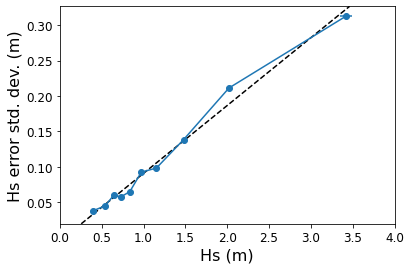
\includegraphics[width = .5\textwidth]{figures/hsobsstd}
\caption{A plot of significant wave height error standard deviation against significant wave height. Calculated using observations from a period spanning 05/10/2021-13/04/2022}
\label{fig:hsobsstd}
\end{figure}

\begin{figure}
\centering
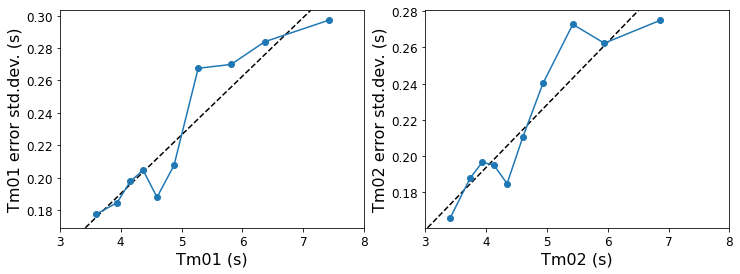
\includegraphics[width = \textwidth]{figures/periodobsstd}
\caption{Plots of $T_{m01}$ and $T_{m02}$ error standard deviation against $T_{m01}$ and $T_{m02}$ respectively.}
\label{fig:periodobsstd}
\end{figure}

Repeating this process with the observations of $T_{m01}$ and $T_{m02}$ yields the plots shown in figure \ref{fig:periodobsstd}. The error distributions for $T_{m01}$ and $T_{m02}$ also fall aproximately on straight lines, though the fit is not as good as for $H_s$. The gradients are also shallower, with the error standard deviations being approximately 3.5\% of the observed variable for both.

Since the error standard deviations match the linear model well, this motivates modelling the error standard deviation in $H_s$ as being equal to 10\% of $H_s$, and the error standard deviation in $T_{m01}$ and $T_{m02}$ as 3.5\% of $T_{m01}$ and $T_{m02}$ respectively. Since the errors in period are such a small percentage of the observations, it is possible that at short periods the error may become very small, which would lead the to DA system fitting the observations too closely and producing physically unrealistic increments. To avoid this, we choose a minimum error threshold $\varepsilon_0$ and set the observation error standard deviation equal to this threshold whenever the scaling method gives a value less than $\varepsilon_0$. This requires estimating a constant scale for the error variance, and methods for doing that are described in the next section.

\subsection{Constant Error Variance}
\label{sec:consterrs}

A simple way to get a constant estimate of error variance is to plot a histogram of observation - ensemble mean, called an $o - b$ plot. The spread in $o - b$ comes from a combination of observation and background error \citep{Desroziers2005}, so a simple way of estimating the observation error is to assume that observation error accounts for a constant proportion of this spread. It is reasonable to assume that the contributions from background and obsevation errors are similarly sized, so the observation error can be estimated to be 50\% of the total spread.

An $o - b$ histogram for significant wave height is shown in figure \ref{fig:hsominusb}. The spread on the histogram is approximately 1m, so the standard deviation of observational errors in significant wave height may be estimated to be approximately 50cm.

Another thing that is visible from the $o-b$ plot is a bias in either the $H_s$ forecasts or observations. The peak of the histogram is centred at around 30cm, which means that the forecast model tends to predict significant wave heights that are about 30cm less than those observed. If this bias is a result of the model, it would be desirable to investigate the capability of DA to reduce this bias. However, with the twin experiment method that is used in this project, this would require introducing an artificial bias to the observations, which is not done in this study (see section \ref{sec:twinexp} for details).

\begin{figure}
\centering
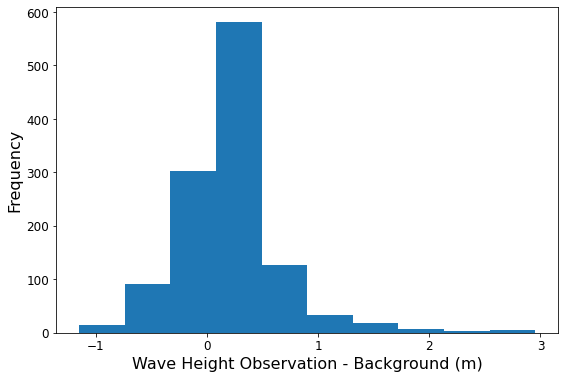
\includegraphics[width = .8\textwidth]{figures/hsominusb}
\caption{Observation - background histogram for significant wave height, from the forecast window 06/03/2022 to 19/03/2022.}
\label{fig:hsominusb}
\end{figure}

\citet{Desroziers2005} provides a more rigorous approach to estimating observational error variances, by defining $\vect{d^o_b} = \y - \mathbf{H}\x_b$ and using the relation

\begin{equation}
\mathbb{E}\left[\vect{d^o_b}\left( \vect{d^o_b} \right)^\top \right] = \mathbf{H} \mathbf{P}^f \mathbf{H}^\top + \mathbf{R}
\end{equation}

Taking traces and dividing by the number of observations gives a good estimate for the average observation error variance $\overline{\text{var} \left( \delta \y_i \right)}$ which is

\begin{equation}
\overline{\text{var} \left( \delta \y_i \right)} = \frac{\text{Tr}(\mat{R})}{\text{\# observations}} \approx \frac{\mathbb{E}\left[ \sum_{i} \left( \vect{d^o_b} \right)_i^2 \right]}{\text{\# observations}} - \frac{\text{Tr}\left( \mathbf{H} \mathbf{P}^f \mathbf{H}^\top \right)}{\text{\# observations}}.
\label{eqn:obserrestimate}
\end{equation}

In our case, the observation operator is very simple and just selects the forecast values from the appropriate location and times, so the diagonal elements of $\mat{H P}^f \mat{H}^\top$ are simply the forecast ensemble variances at the observation location and times. To determine the minimum error threshold, the estimate in equation \ref{eqn:obserrestimate} is evaluated using only the observations of period with a value of less than 5 seconds, as these are the observations which may lead to excessively small errors. The terms on the right hand side of \ref{eqn:obserrestimate} are found to be

\[
\frac{\mathbb{E}\left[ \sum_{i} \left( \vect{d^o_b} \right)_i^2 \right]}{\text{\# observations}} = 0.29 \, \text{s}^2, \quad \frac{\text{Tr}\left( \mathbf{H} \mathbf{P}^f \mathbf{H}^\top \right)}{\text{\# observations}} = 0.17 \, \text{s}^2
\]

So the observation error variance is estimated to be $0.29 \, \text{s}^2 - 0.17 \, \text{s}^2 = 0.12 \, \text{s}^2$ and the standard deviation threshold is set at $\sqrt{0.12 \, \text{s}^2} = 0.35 \text{s}$. Examining the $o-b$ histograms for $T_{m01}$ and $T_{m02}$ in figure \ref{fig:periodominusb} confirms that this is a sensible value to choose.

\begin{figure}[h]
\centering
\begin{subfigure}{.45\textwidth}
\centering
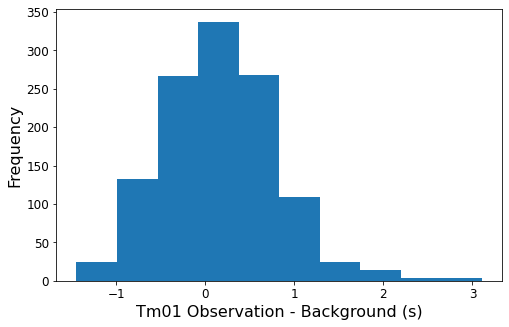
\includegraphics[width = \textwidth]{figures/tm01ominusb}
\end{subfigure}
\begin{subfigure}{.45\textwidth}
\centering
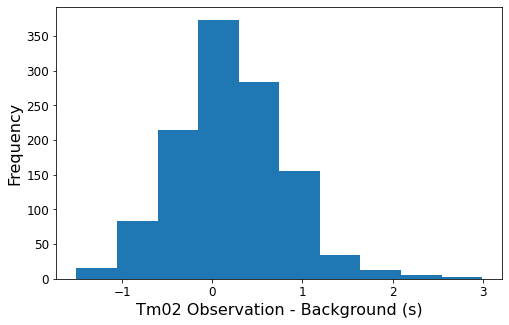
\includegraphics[width = \textwidth]{figures/tm02ominusb}
\end{subfigure}
\caption{Observation minus background histograms for $T_{m01}$ (left) and $T_{m02}$ (right).}
\label{fig:periodominusb}
\end{figure}

In this section, we have found that the observation error standard deviations in all variables are strong functions of the observed values, with the error in $H_s$ being approximately 9.6\% of the observed value and the error in both periods being approximately 3.5\% of the observation.

Motivated by this, the $H_s$ error is set to 10\% of the observed value in the assimilation of significant wave height alone. For the assimilation of all variables, there is more risk of fitting the observations too closely as more observations are assimilated. Because of this, the scales of error standard deviation are increased from those found above to 12\% for significant wave height and 7\% for the periods. A minimum error threshold of $0.35s$ is implemented for the periods.

\section{Chapter Summary}

In this chapter we have given characterisations of the background and observation errors. Knowledge of these errors is vital to DA as between them they control a large part of the workings of a DA system. The results shown in this chapter are intended to aid understanding of the results of the DA experiments, which are presented in the next chapter.
